\documentclass[12pt, a4paper, twocolumn]{article}
\pdfoutput=1
\pdfminorversion=4

\usepackage[T1]{fontenc}
\usepackage[utf8]{inputenc}
\usepackage[english]{babel}
\usepackage{units}
\usepackage{graphicx}
\usepackage{lmodern}
\usepackage{color}

\usepackage{hyperref}



\usepackage{physics}

\usepackage[english,iso]{isodate}



\graphicspath{ {Figures/} }

\usepackage[margin=10pt, font=small]{caption}
%\usepackage{todonotes} %\todo{...}, \todolist







\begin{document}

\title{Measuring $g$ using a rotating liquid mirror:
  Enhancing laboratory learning} 

\newcommand{\andsunds}{andsunds@chalmers.se}
\author{Andréas Sundström\footnote{Engineering Physics, Chalmers
    University of Technology, Gothenburg, Sweden,
    \textcolor{blue}{\href{mailto:\andsunds}{\nolinkurl{\andsunds}}} }
\and Tom Adawi\footnote{Engineering Education Research, Chalmers
  University of Technology, Gothenburg, Sweden} 
}
\date{Accepted 2016-05-10}
\maketitle

\begin{abstract}
We describe a low-cost yet experimentally challenging method to measure the acceleration of gravity, $g$, using a liquid in a rotating bowl and a laser pointer. The idea underpinning this novel method is that the rotating liquid surface will form a parabolic reflector which will focus light into a unique focal point. By measuring the height of the focal point, $g$ could be determined to $\unit[9.78 \pm 0.13]{m/s^2}$. We discuss the pedagogical merits of this method compared to more traditional methods for measuring $g$, and how it can be implemented as an experimental problem at different educational levels. 
\end{abstract}


\section{Introduction}

The acceleration of gravity, $g$, has been measured countless times in secondary school and undergraduate physics laboratories. This is usually done through some sort of pendulum or free fall experiment. In terms of experimental \emph{simplicity} these methods are hard to beat. On the other hand, these methods do not excite much experimental \emph{creativity}. In these cookbook labs, the students follow step-by-step instructions and there is little room for intellectual engagement~\cite{Wieman2015}. As pointed out by Germann et al.~\cite{Germann1996}, 
``Recipe-like activities often short circuit opportunities to stimulate thinking by students''. 
Consequently, cookbook labs have basically no impact on students' understanding of the nature and practice of science~\cite{Domin1999}. 

In this paper, we describe a novel and more thought-provoking way to measure the acceleration of gravity. The main idea of the method is to study the surface of a liquid in a rotating bowl. The surface will form a \emph{parabolic reflector}~\cite{Berg1990}, which will focus incoming planar light. In the next section we show that the focal point of the parabolic reflector is located at the height
\begin{equation}\label{eq:g}
h=\frac{g}{2\omega^2}
\end{equation}
above the vertex, where $\omega$ is the angular frequency of the bowl. By locating the focal point with a laser pointer, the value of $g$ can be determined. Since only the focal height and the angular frequency will influence the value of $g$ this method is experimentally quite clean, with only two parameters to measure. 

Since there are many ways to locate the focal point, for example, the proposed method can stimulate the students' experimental creativity. Moreover, the students are encouraged to combine their knowledge from two areas of physics -- mechanics and optics. Michael Faraday said: 
``I was never able to make a fact my own without seeing it''.
Hence an additional pedagogical benefit of the proposed method, is that students actually get to \emph{see} the focal point of a parabolic reflector (see Figure 2). In this way, the proposed experiment to measure $g$ addresses the three fundamental objectives of laboratory instruction as defined by Ernst:
``First, the student should learn how to be an experimenter. Second, the laboratory can be a place for the student to learn new and developing subject matter. Third, laboratory courses help the student to gain insight and understanding of the real world''~\cite{Ernst1983}.

A somewhat similar method for measuring the acceleration of gravity has been used as part of an experimental problem in the International Physics Olympiad, IPhO~\cite{IPhO2001}. However, in the IPhO problem a different aspect of the parabolic surface was used to determine $g$. They used the fact that the surface, in a rotating cylindrical vessel, will not change its height at a certain distance from the center, independent of rotational speed. Apart from this, we have not been able to find any previous reports of experiments that use a rotating liquid surface to determine the acceleration of gravity.

\section{Theory}
We derive our central equation~\eqref{eq:g} in two steps. First, we show that the top surface of a liquid in a rotating cylindrical vessel will form a \emph{paraboloid}. We then derive an equation for the \emph{focal length} of this parabolic surface.

\begin{figure}\centering
\resizebox{7.5cm}{!}{\begin{picture}(0,0)%
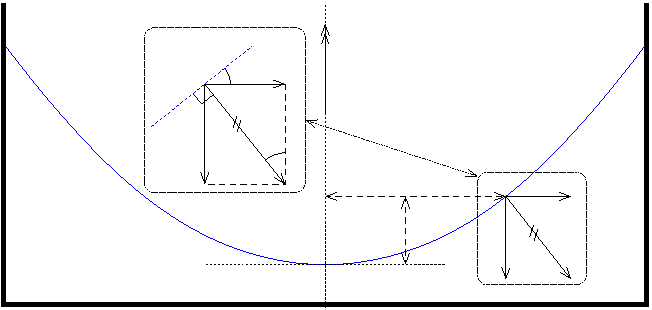
\includegraphics{fig1_parabola.pdf}%
\end{picture}%
\setlength{\unitlength}{2818sp}%
%
\begingroup\makeatletter\ifx\SetFigFont\undefined%
\gdef\SetFigFont#1#2#3#4#5{%
  \reset@font\fontsize{#1}{#2pt}%
  \fontfamily{#3}\fontseries{#4}\fontshape{#5}%
  \selectfont}%
\fi\endgroup%
\begin{picture}(7288,3476)(-43,-3043)
\put(6250,-2450){\makebox(0,0)[lb]{\smash{{\SetFigFont{18}{14.4}{\familydefault}{\mddefault}{\updefault}{\color[rgb]{0,0,0}$a$}%
}}}}
\put(5401,-2581){\makebox(0,0)[lb]{\smash{{\SetFigFont{14}{14.4}{\familydefault}{\mddefault}{\updefault}{\color[rgb]{0,0,0}$g$}%
}}}}
\put(5940,-1680){\makebox(0,0)[lb]{\smash{{\SetFigFont{14}{14.4}{\familydefault}{\mddefault}{\updefault}{\color[rgb]{0,0,0}$a_c$}%
}}}}
\put(3700,-100){\makebox(0,0)[lb]{\smash{{\SetFigFont{18}{14.4}{\familydefault}{\mddefault}{\updefault}{\color[rgb]{0,0,0}$\omega$}%
}}}}
\put(4300,-1681){\makebox(0,0)[lb]{\smash{{\SetFigFont{16}{14.4}{\familydefault}{\mddefault}{\updefault}{\color[rgb]{0,0,0}$r$}%
}}}}
\put(4546,-2100){\makebox(0,0)[lb]{\smash{{\SetFigFont{16}{14.4}{\familydefault}{\mddefault}{\updefault}{\color[rgb]{0,0,0}$z(r)$}%
}}}}
%v-- the small insert --v
\put(1980,-1456){\makebox(0,0)[lb]{\smash{{\SetFigFont{18}{14.4}{\familydefault}{\mddefault}{\updefault}{\color[rgb]{0,0,0}$g$}%
}}}}
\put(2880,-1231){\makebox(0,0)[lb]{\smash{{\SetFigFont{17}{14.4}{\familydefault}{\mddefault}{\updefault}{\color[rgb]{0,0,0}$\alpha$}%
}}}}
\put(2566,-450){\makebox(0,0)[lb]{\smash{{\SetFigFont{17}{14.4}{\familydefault}{\mddefault}{\updefault}{\color[rgb]{0,0,0}$\alpha$}%
}}}}
\put(2900,-376){\makebox(0,0)[lb]{\smash{{\SetFigFont{18}{14.4}{\familydefault}{\mddefault}{\updefault}{\color[rgb]{0,0,0}$a_c$}%
}}}}
\end{picture}%
}
\caption{Cross section of the liquid surface in a rotating vessel. The surface will be perpendicular to the net acceleration in the rotating frame of reference. Since the centrifugal acceleration will increase linearly with $r$, so will the slope of the surface ${\nicefrac{\dd{z}}{\dd{r}}=\tan\alpha}$. }
\label{fig:parabola} 
\end{figure}

By studying the centrifugal acceleration in the rotating frame of reference alongside gravity, we see from Figure~\ref{fig:parabola} that the angle $\alpha$ of the surface depends on $g$ and the centrifugal acceleration $a_c$ as $\tan\alpha=a_c/g$. To obtain the full relationship, we first note that the surface of a freely flowing liquid will be perpendicular to the perceived net acceleration. Then we note that the derivative of a function is equal to the tangent of the angle to the horizontal line, whereby we get an expression for the derivative of the slope of the surface in Figure~\ref{fig:parabola}:
\begin{equation}\label{eq:slope}
\dv{z}{r} = \tan\alpha = \frac{a_c}{g}.
\end{equation}
With the centrifugal acceleration $a_c=r\omega^2$, the equation for the surface can be found by integrating the left and right hand side of~\eqref{eq:slope}: 
\begin{equation}\label{eq:parabola}
z(r)=\frac{r^2\omega^2}{2g}.
\end{equation}
This is the equation for a \emph{parabolic} surface. \v{S}abatka and Dv\v{o}rák~\cite{Sabatka2010} have described a simple experiment to verify the parabolic shape of a liquid in a rotating cylindrical vessel. 

\begin{figure}\centering
\resizebox{4cm}{!}{\begin{picture}(0,0)%
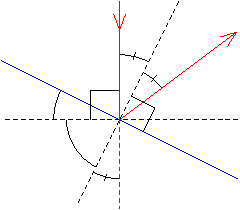
\includegraphics{fig2_angles.pdf}%
\end{picture}%
\setlength{\unitlength}{4144sp}%
%
\begingroup\makeatletter\ifx\SetFigFont\undefined%
\gdef\SetFigFont#1#2#3#4#5{%
  \reset@font\fontsize{#1}{#2pt}%
  \fontfamily{#3}\fontseries{#4}\fontshape{#5}%
  \selectfont}%
\fi\endgroup%
\begin{picture}(1824,1599)(439,-523)
\put(676,254){\makebox(0,0)[lb]{\smash{{\SetFigFont{14}{16.8}{\familydefault}{\mddefault}{\updefault}{\color[rgb]{0,0,0}$\alpha$}%
}}}}
\put(1171,-438){\makebox(0,0)[lb]{\smash{{\SetFigFont{14}{16.8}{\familydefault}{\mddefault}{\updefault}{\color[rgb]{0,0,0}$\gamma$}%
}}}}
\put(824,-174){\makebox(0,0)[lb]{\smash{{\SetFigFont{14}{16.8}{\familydefault}{\mddefault}{\updefault}{\color[rgb]{0,0,0}$\beta$}%
}}}}
\put(1441,704){\makebox(0,0)[lb]{\smash{{\SetFigFont{14}{16.8}{\familydefault}{\mddefault}{\updefault}{\color[rgb]{0,0,0}$\gamma$}%
}}}}
\end{picture}%
}
\caption{
The water surface with the incoming and reflected light. Since the angles in the figure sums to $\alpha+\beta= 90^\circ = \gamma+\beta$, the angle between the incoming light and the normal to the surface will be~$\gamma=\alpha$. }
\label{fig:angles} 
\end{figure}

\begin{figure*}
\centering
\resizebox{9cm}{!}{\begin{picture}(0,0)%
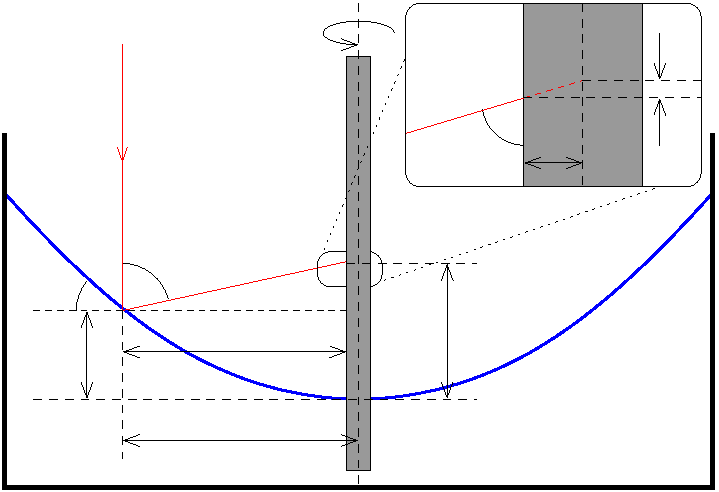
\includegraphics{fig3_rot_bowl.pdf}%
\end{picture}%
\setlength{\unitlength}{4144sp}%
%
\begingroup\makeatletter\ifx\SetFigFont\undefined%
\gdef\SetFigFont#1#2#3#4#5{%
  \reset@font\fontsize{#1}{#2pt}%
  \fontfamily{#3}\fontseries{#4}\fontshape{#5}%
  \selectfont}%
\fi\endgroup%
\begin{picture}(5466,3735)(418,-3694)
\put(3916,-2536){\makebox(0,0)[lb]{\smash{{\SetFigFont{17}{20.4}{\familydefault}{\mddefault}{\updefault}{\color[rgb]{0,0,0}$\hat{h}$}%
}}}}
\put(1576,-1996){\makebox(0,0)[lb]{\smash{{\SetFigFont{17}{20.4}{\familydefault}{\mddefault}{\updefault}{\color[rgb]{0,0,0}$2\alpha$}%
}}}}
\put(1801,-2581){\makebox(0,0)[lb]{\smash{{\SetFigFont{17}{20.4}{\familydefault}{\mddefault}{\updefault}{\color[rgb]{0,0,0}$\hat{r}=(r-\rho)$}%
}}}}
\put(1936,-3256){\makebox(0,0)[lb]{\smash{{\SetFigFont{17}{20.4}{\familydefault}{\mddefault}{\updefault}{\color[rgb]{0,0,0}$r$}%
}}}}
\put(856,-2176){\makebox(0,0)[lb]{\smash{{\SetFigFont{17}{20.4}{\familydefault}{\mddefault}{\updefault}{\color[rgb]{0,0,0}$\alpha$}%
}}}}
\put(631,-2716){\makebox(0,0)[lb]{\smash{{\SetFigFont{17}{20.4}{\familydefault}{\mddefault}{\updefault}{\color[rgb]{0,0,0}$z(r)$}%
}}}}
\put(5491,-421){\makebox(0,0)[lb]{\smash{{\SetFigFont{17}{20.4}{\familydefault}{\mddefault}{\updefault}{\color[rgb]{0,0,0}$\delta$}%
}}}}
\put(4591,-1096){\makebox(0,0)[lb]{\smash{{\SetFigFont{17}{20.4}{\familydefault}{\mddefault}{\updefault}{\color[rgb]{0,0,0}$\rho$}%
}}}}
\put(3961,-1141){\makebox(0,0)[lb]{\smash{{\SetFigFont{17}{20.4}{\familydefault}{\mddefault}{\updefault}{\color[rgb]{0,0,0}$2\alpha$}%
}}}}
\put(2791,-466){\makebox(0,0)[lb]{\smash{{\SetFigFont{17}{20.4}{\familydefault}{\mddefault}{\updefault}{\color[rgb]{0,0,0}$\omega$}%
}}}}
\end{picture}%
}
\caption{
Schematic drawing of the setup together with the definitions of the notation used in the calculations. Due to the focal height being measured slightly outside the exact center of the rod, by $\rho$, a small correction $\delta$ has to be made to the measured focal height.} 
\label{fig:rot_bowl} 
\end{figure*}

To find the focal length of the parabolic surface, we begin by studying Figure~\ref{fig:angles}. Since we have two right angles, between on the one hand the incoming light and the horizontal line and on the other hand between the surface and the normal, both 
$\alpha+\beta = 90^\circ$ and $\gamma+\beta = 90^\circ$. 
Therefore the total angle between the incoming and reflected light is $2\alpha$. 

Furthermore, we see from Figure~\ref{fig:rot_bowl} that the point where the reflected light crosses the axis of rotation is at the height 
\begin{equation}
h= z(r) + r\,\cot(2\alpha)
\end{equation}
above the vertex of the parabola. We now use the equations in \eqref{eq:slope} and \eqref{eq:parabola} together with the trigonometric identity
\begin{equation}
\begin{aligned}
\cot(2\alpha)
&=\frac{\cos^2\alpha-\sin^2\alpha}{2\,\cos\alpha\,\sin\alpha}\\
&=\frac{\cos\alpha}{2\sin\alpha}-\frac{\sin\alpha}{2\cos\alpha}\\
&=\frac{1}{2}\left(\frac{1}{\tan\alpha} -\tan\alpha \right),
\end{aligned}
\end{equation}
to obtain
\begin{equation}\label{eq:focal_height}
h=\frac{r^2\omega^2}{2g} 
   + \frac{r}{2}\left(\frac{g}{r\omega^2} -\frac{r\omega^2}{g} \right)
=\frac{g}{2\omega^2}.
\end{equation}
This is the \emph{focal length} of our parabolic surface, and the equation that we set out to derive. Note that $h$ is \emph{independent} of $r$ (and $\alpha$). In other words, a parabolic surface has a \emph{unique} focal point.

\section{Experimental setup}

The experimental set up shown in Figure~\ref{fig:rot_bowl_pic} consists of a bowl of water on a spinning disk, a laser pointer, a central rod marking out the axis of rotation, and a photo-diode for measuring the speed of rotation. The spinning disk was powered by a DC motor so the rotational speed could be adjusted by varying the voltage applied to the motor. 

The focal point will be located somewhere along the axis of rotation. When shining a laser vertically down at the parabolic surface, the refection will hit the central rod at the height $h$ over the vertex, which can be measured using a narrow ruler. 

By varying the rotational speed and measuring the focal height for different speeds, a linear regression could be made for $g$ as the slope of the curve of $h$ plotted against $1/(2\omega^2)$.  Measurements were taken at two different radial distances from the center to verify that the radial distance has no impact on the measured value of $g$. 

The rotational speed, $\omega$, was measured with a photo-diode connected to a digital oscilloscope which could record several periods of rotation. A more readily available option is to connect the photo-diode to a computer's microphone input and record the signal as a ``sound'' file on the computer, as in~\cite{Sabatka2010}. Since $\omega$ is one of the two parameters directly determining the value of $g$, it's recommended to measure the periods with some kind of digital logging device, such as an oscilloscope or computer, to minimize uncertainty in this parameter.

\begin{figure}
\centering
\resizebox{6cm}{!}{\begin{picture}(0,0)%
\includegraphics{fig4_rot_bowl_pic.pdf}%
\end{picture}%
\setlength{\unitlength}{4144sp}%
%
\begingroup\makeatletter\ifx\SetFigFont\undefined%
\gdef\SetFigFont#1#2#3#4#5{%
  \reset@font\fontsize{#1}{#2pt}%
  \fontfamily{#3}\fontseries{#4}\fontshape{#5}%
  \selectfont}%
\fi\endgroup%
\begin{picture}(24203,34432)(676,-34943)
\put(12916,-11266){\makebox(0,0)[lb]{\smash{{\SetFigFont{150}{180.0}{\familydefault}{\mddefault}{\updefault}{\color[rgb]{0,0,0}Focus}%
}}}}
\end{picture}%
}
\caption{A photograph of the setup running. The reflected beam from a laser pointer (outside frame) can be seen at the focal point on the central rod. %The arm blocking the light to the photodiode can be seen as a blur in the lower left corner.
} 
\label{fig:rot_bowl_pic} 
\end{figure}


\subsection{Calibration}

The laser pointer has to be perfectly vertical. This calibration can be done by shining the laser down on the water surface when it's not rotating. The laser-beam will be perfectly vertical when the reflection hits the source.

To get the central rod centered, a center mark was put in the rotating disc. A spirit level was used to ensure that the central rod was vertical. Both of these steps are essential, since deviation from the center will change the measured value of $g$, as we will see in next section. 


\subsection{Correction}\label{sec:corrections}

As shown in Figure~\ref{fig:rot_bowl}, the measured focal height $\hat{h}$ is slightly off from the real focal height by 
\begin{equation}%\label{eq:correction}
\delta=\rho\cot 2\alpha
\end{equation}
due to a finite width, $\rho$, of the central rod. This width is easily measured with a pair of calipers.

We now have to determine $\alpha$. First, we remember that
\begin{equation}\label{eq:dz/dr}
\tan\alpha=\dv{z}{r} =\frac{2 z(r)}{r}.
\end{equation}
Then, we can see from Figure~\ref{fig:rot_bowl} that 
\begin{equation}
\cot 2\alpha =\frac{\hat{h} - z(r)}{\hat{r}} 
= \frac{\hat{h}-\frac{r}{2}\tan\alpha }{\hat{r}},
\end{equation}
where we used \eqref{eq:dz/dr} to substitute $z(r)$ in terms of $\tan\alpha$. By rewriting the last equation, we get
\begin{equation}
\cot 2\alpha 
-\frac{\hat{h}}{\hat{r}}
+\frac{\hat{r}+\rho}{2\hat{r}}\tan\alpha  = 0.
\end{equation}
This expression consists of known or measured quantities and $\alpha$. From this stage, $\alpha$ can easily be obtained to a satisfying degree with regular numerical equation solvers.


\section{Results and discussion}

The results from the measurements together with the least square fit are shown in Figure~\ref{fig:data}. The calculated value of the acceleration of gravity comes out as
\begin{equation}
g=\unit[9.78\pm 0.13]{m/s^2}.
\end{equation}
The uncertainty given is the standard error in the mean.

\begin{figure*}\centering 
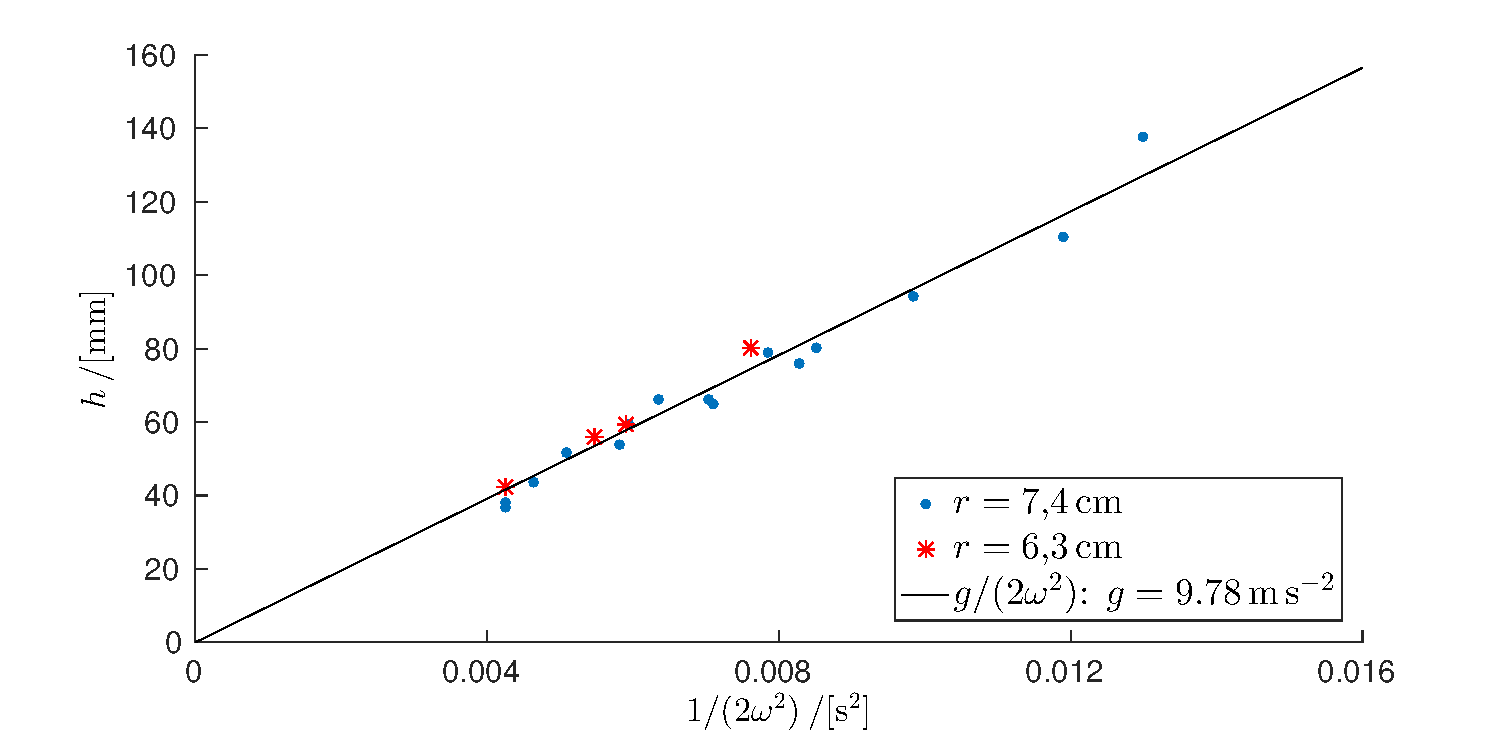
\includegraphics[width=12cm]{fig5_data.pdf}
\caption{
Measurements of the focal height $h$ (with corrections for a center rod of non-zero width) plotted against $1/(2\omega^2)$. The acceleration of gravity $g$ is given as the slope of the least square fit to these data points. Measurements were taken at two different radial distances, $r$, from the center.}
\label{fig:data} 
\end{figure*}

Since this is a new method for measuring $g$, it is not easy to compare our result to those by others. The closest comparison we can make is to the results from the experimental part in the IPhO in 2001~\cite{IPhO2001}. There, it is stated that $g$ could be measured to $\unit[9.8]{m/s^2}$ with a standard error of $\unit[0.2]{m/s^2}$. So our result seems to be at least as good, or perhaps even a little better, compared to those obtained through other methods using a rotating liquid. 

The error in our method is, however, considerably larger than the error in some of the most sophisticated pendulum methods~\cite{Candela2001}. But as mentioned in the introduction, the proposed method has several pedagogical advantages compared to more traditional methods for measuring $g$. Apart from encouraging experimental creativity, this method encourages students to consider experimental corrections. 

The significance of the correction, $\delta$, due to the finite width of the central rod is quite notable. The value of $g$ comes out to be only about $\unit[9.2]{m/s^2}$ \emph{without} these corrections. This demonstrates the necessity of the calculations made in section~\ref{sec:corrections}. 

Although the proposed method for measuring $g$ is new, the focusing property of a rotating liquid surface has been used before. Berg~\cite{Berg1990} used this property to focus light into an optical image, while Graumann and Laue~\cite{Graumann1998} described several optics experiments involving a rotating liquid surface. 
There are even telescopes today that use a rotating pool of mercury as the mirror to get a perfect parabolic reflector~\cite{Shiga2008}.

\subsection{Experimental improvements}

Most of the uncertainty in the result is due to small ripples on the water surface, leading to a jittery motion of the reflected laser beam. Both Berg~\cite{Berg1990} and the IPhO~\cite{IPhO2001} experimental problem used glycerin as the liquid. Due to the high viscosity of glycerin, there will be less ripples on the surface.

Another way to increase the accuracy would be to use a bigger bowl, preferably one with vertical walls. The maximal rotational speed will be limited by the slope of the walls, since the walls have to have a steeper slope than the water surface.

Finally, there are other ways to locate the focal point. For example, two different lasers could be used. By shining the two laser beams vertically down at two different points at the rotating surface, the focus can then be located at the point of intersection of the reflected beams. Note that this will eliminate the need to calculate the correction in section~\ref{sec:corrections}. 

\subsection{Pedagogical reflections}

The experiment to measure the acceleration of gravity described in
this paper could be carried out as a shorter project for secondary
school students or as a laboratory exercise for first-year
undergraduate physics students. One should note though, that the
experiment takes around 2--4~hours from scratch to finished
measurements, depending on the desired experimental accuracy. If this
experiment is conducted as a project, the students could compare this
method to more traditional methods for measuring the acceleration of
gravity.

Traditional laboratory instruction has been criticized for the
emphasis it places on following step-by-step instructions, leaving
little room for intellectual engagement~\cite{Wieman2015}. In these
cookbook labs, ``virtually no attention is given to the planning of
the investigation or to interpreting the
results''~\cite{Domin1999}. As a consequence, ``virtually no
meaningful learning takes place''~\cite{Domin1999}. As a way to avoid
the cookbook-style lab exercise, the method for measuring the
acceleration of gravity described in this paper could form the basis
for a more open experimental problem. The students could, for example,
be asked to determine the acceleration of gravity using some given
equipment. But as always when there is no ``recipe'' to follow,
unintended solutions might appear – like the one
in~\cite{IPhO2001}. This is, however, not necessarily a bad thing. As
Pickering noted, in cookbook labs, students are never ``forced to
reconcile results, or confronted with challenge to what is naively
predictable''~\cite{Pickering1987}.

The instruction to determine something using a given set of equipment
and with no further information regarding the procedure, is common in
physics competitions, like the IPhO. An experimental problem with this
type of minimal instruction, might therefore be more suited for
students who already have a good understanding of physics. Although
this type of minimal instruction is common in the IPhO, the
experimental problem in 2001~\cite{IPhO2001} included quite a few
hints. This indicates that the concept of measuring the acceleration
of gravity with a rotating liquid surface could be too challenging for
most secondary school students without additional guidance. The hints
provided in the IPhO experimental problem in 2001 could be used as a
source of inspiration for developing laboratory instructions suitable
for students with different levels of background knowledge and at
different educational levels. 

\section{Conclusion}

In this paper, we have described a novel method for measuring the acceleration of gravity. As an \emph{experimental} method, it fares well compared to similar methods~\cite{IPhO2001}, but not as well compared to some of the most accurate methods~\cite{Candela2001}. 

As a \emph{pedagogical} method, it holds great potential to enhance laboratory learning. The overall aim was to break away from the cookbook lab and engage students in more authentic scientific thinking. With suitable scaffolding, the proposed method allows students to combine knowledge from two areas of physics, mechanics and optics, and develop important skills, including experimental creativity. Moreover, students get to see the focusing property of parabolic mirrors while doing this experiment.

\section*{Acknowledgments}

We are very grateful to the personnel in the machine shop at the
Physics Department at Chalmers. We thank Lars Hellberg and Jan-Åke
Wiman for constructing and balancing the rotating disk so that the
experiments could be performed. 

We would also like to thank Johan Runeson who, together with Andréas
Sundström, in the late spring of 2015 performed the measurements and
laboratory work for this article. 

%Bibliography
\bibliographystyle{unsrt}
\bibliography{bibliography}

\end{document}